% Chapter 1

\chapter{Introducción general} % Main chapter title

\label{Chapter1} % For referencing the chapter elsewhere, use \ref{Chapter1} 
\label{IntroGeneral}

%----------------------------------------------------------------------------------------

% Define some commands to keep the formatting separated from the content 
\newcommand{\keyword}[1]{\textbf{#1}}
\newcommand{\tabhead}[1]{\textbf{#1}}
\newcommand{\code}[1]{\texttt{#1}}
\newcommand{\file}[1]{\texttt{\bfseries#1}}
\newcommand{\option}[1]{\texttt{\itshape#1}}
\newcommand{\grados}{$^{\circ}$}

%----------------------------------------------------------------------------------------

%\section{Introducción}

En este capítulo se brinda mayor detalle sobre la importancia del trabajo realizado y sus beneficios para el Banco de Crédito del Perú. Adicionalmente, se especifica cuál es el objetivo y el alcance del proyecto. Finalmente, se brinda un breve resumen de los avances tecnológicos más recientes en inteligencia artificial generativa y los retos implicados en su uso.

%----------------------------------------------------------------------------------------
\section{Motivación}

Uno de los principales medios de comunicación dentro del Banco de Crédito del Perú (BCP) es el email. Dentro de la organización existen varios equipos que usan esta herramienta para comunicar campañas a los clientes, promociones, brindar consejos financieros, entre otros objetivos diversos por áreas. Sin embargo, el proceso de creación de los emails maquetados puede tomar entre 5 a 8 días hábiles, y el equipo que recibe estos pedidos tiene capacidad limitada, por lo que se deben priorizar y rechazar algunas solicitudes. Adicionalmente, estos emails son estáticos y difíciles de personalizar por la carga que conlleva realizar artes diferentes. Esto dificulta comunicar a los clientes de forma oportuna, con la frecuencia deseada y con mayor personalización. Además, vuelve complejo el realizar experimentos y campañas que exigen el uso de bocetos variados para diferentes grupos de clientes, o la actualización continua del contenido de los correos electrónicos. 

En la figura~\ref{fig:procesoEmail}, se resumen los pasos para la creación de un correo electrónico tal cual se realizan en la empresa previo al desarrollo de este trabajo. 

\begin{landscape}
\begin{figure}[htbp]
\centering
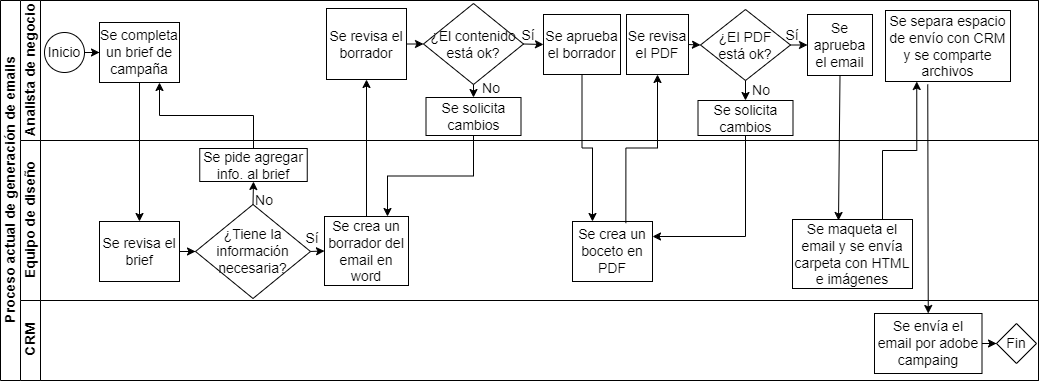
\includegraphics[width=\linewidth]{./Figures/Diagrama1_Creacion_Emails.png}
\caption{Proceso de creación de emails para clientes.}
\label{fig:procesoEmail}
\end{figure}
\end{landscape}

Como se puede observar, es un flujo largo que tiene muchas oportunidades de optimización. Este proceso inicia con la solicitud de creación de un email por parte de algún analista de negocio, el cual crea un \textit{brief} que es un documento que incluye el objetivo del correo, el contenido, público objetivo y otras instrucciones necesarias para su desarrollo. El equipo de diseño revisa este archivo y crea inicialmente un borrador del texto que se incluirá en el email. Tras su aprobación, recién inicia la maquetación del correo electrónico en HTML. Entre estos pasos, existen varias idas y vueltas entre ambos equipos para hacer correcciones en los bocetos que le toman al equipo de diseño varios días.

Sin embargo, gracias al avance de la inteligencia artificial (IA) generativa este proceso se puede reducir a unos pocos minutos, lo cual hace posible que las campañas comerciales y comunicación relacional sean enviadas a tiempo a los clientes. Además, se liberará de carga al equipo de diseño de tal forma que pueda enfocarse en actividades más creativas y que generen más valor a la organización. Esto implicará tanto ahorro de costos para la empresa como incremento en ventas gracias a la mejora en la comunicación comercial.

%----------------------------------------------------------------------------------------

\section{Objetivos y alcance}

El objetivo del trabajo propuesto es agilizar el proceso de creación de emails del Banco de Crédito del Perú y minimizar el esfuerzo humano mediante el uso de inteligencia artificial generativa. Estos correos deben crearse respetando los lineamientos de marca de la empresa, el estilo que corresponde a cada segmento de clientes del banco y deben aplicar correctamente la terminología bancaria.

\subsection{Alcance}

Este trabajo incluye una solución tecnológica en base a inteligencia artificial que pueda entender la información escrita en lenguaje natural brindada dentro de un \textit{brief} y, a partir de este, generar un email compuesto por texto e imágenes. Este email puede ser previsualizado por el usuario para permitir su revisión y aprobación. Una vez aprobado el diseño, el \textit{output} final que se comparte al solicitante es una carpeta con el archivo HTML y las imágenes necesarias.

Dentro de la solución brindada se incluyen las funcionalidades para poder pedir modificaciones sobre el documento HTML ya generado y poder adaptar el estilo a segmentos de clientes Bex y Enalta. Adicionalmente, se ha desarrollado una interfaz sencilla para que los usuarios no técnicos puedan usar el modelo.

El presente trabajo no incluye ninguna conexión directa con Adobe Campaign, que es la herramienta utilizada por la empresa para el envío de correos electrónicos. Tampoco está dentro del alcance la generación de emails para clientes corporativos del banco o correos con contenido de productos para empresas. Además, quedan pendientes las siguientes funcionalidades para futuros desarrollos: 

\begin{itemize}
    \item Poder incluir archivos \textit{GIF (Graphic Interchange Format)} dentro del email.
    \item Adaptar el estilo a segmentos de clientes Enalta y Banca Privada.
    \item Poder personalizar secciones del mail (como frases o imágenes) según \textit{clusters} de clientes específicos.
    \item Entre otras funcionalidades.
\end{itemize}

%----------------------------------------------------------------------------------------

\section{Estado del arte}

El desarrollo de la inteligencia artificial generativa ha sido rápido y disruptivo desde la publicación del influyente \textit{paper} \textit{Attention is All You Need} \citep{Vaswani2017} en 2017. En este se introdujo los transformadores, una arquitectura que ha revolucionado la forma en que las máquinas entienden y generan lenguaje humano y otros tipos de datos. Este método se basa exclusivamente en mecanismos de atención y prescinde de operaciones recurrentes en el procesamiento del lenguaje natural (NLP) \citep{Vaswani2017}. Esto permite a los modelos aprender relaciones complejas en datos de secuencia con mayor eficacia y eficiencia.

Gracias a eso, en 2018, casi simultáneamente, OpenAI y Google lanzaron GPT \citep{Radford2018} y BERT \citep{Devlin2018}, respectivamente. Estos modelos basados en transformadores mostraron capacidades superiores en muchas tareas de procesamiento del lenguaje natural. GPT, en particular, fue diseñado para la generación de texto \citep{Radford2018}, mientras que BERT se centró en mejorar la comprensión del contexto del lenguaje \citep{Devlin2018}.

Desde 2019, OpenAI ha seguido desarrollando y perfeccionando las versiones de GPT, que incluyen GPT-2 y GPT-3, este último lanzado en 2020. En sus inicios, estos modelos fueron utilizados principalmente por desarrolladores, ya que todavía no existía un producto diseñado para el público general. La versión de ChatGPT que se popularizó ampliamente, con una interfaz gráfica amigable para el usuario final, fue lanzada por OpenAI en noviembre de 2022. Esta versión fue específicamente optimizada para interacciones en forma de diálogo y diseñada para ser segura, fácil de usar y accesible para el uso masivo \citep{OpenAI2022ChatGPT}.

Los modelos de lenguaje de gran escala como GPT-3, lanzados durante este período, demostraron capacidades asombrosas como la generación de texto que puede ser indistinguible del escrito por humanos. El interés y la utilización de estos modelos se masificaron rápidamente, impulsados por su aplicación en una amplia gama de industrias, desde asistentes virtuales hasta herramientas de creación de contenido \citep{V7Labs2023}.

Entre las aplicaciones más interesantes de estos modelos están las herramientas de generación de código como GitHub Copilot \citep{GitHubCopilot2023}. Estas utilizan variantes de GPT-3 para ayudar a los desarrolladores a escribir código más rápido y con menos errores. Entre sus capacidades están autocompletar líneas de código, sugerir implementaciones completas de funciones y proporcionar ejemplos de código en tiempo real \citep{GitHubCopilot2023}. 

Por otro lado, en el campo de la generación de imágenes han surgido modelos basados en técnicas de difusión y GANs como DALL-E, Midjourney y Stability AI. Estos han mostrado cómo la IA puede crear imágenes artísticas y realistas a partir de descripciones textuales, revolucionando campos como el diseño gráfico y la moda \citep{BattleOfCreativity2024}.

Estos avances están cambiando la manera de trabajar, ya que permiten mayor eficiencia y nuevas formas de creatividad. La IA generativa sigue evolucionando, prometiendo aún más aplicaciones y mejoras en el futuro. Sin embargo, pese a sus impresionantes capacidades, no está exenta de desafíos y limitaciones. Algunos de los defectos más notables que se deben considerar al aplicarla en diversos desarrollos, son los siguientes \citep{TowardsAI2024}:

\begin{itemize}
    \item Sensibilidad a los \textit{prompts}: Los modelos generativos son altamente sensibles a la forma en que se estructuran los \textit{prompts} o instrucciones. Pequeñas variaciones en el texto pueden llevar a resultados significativamente diferentes. Esto requiere que los usuarios a menudo tengan que experimentar con diferentes formulaciones de \textit{prompts} para alcanzar el resultado deseado.
    \item Inconsistencias y errores fácticos: Los modelos pueden generar información que es inconsistente o incluso incorrecta. Esto es especialmente problemático en aplicaciones que requieren alta precisión factual, como en el ámbito médico o jurídico.
    \item Sesgos en los datos: Los modelos generativos aprenden de grandes volúmenes de datos y pueden heredar y perpetuar los sesgos presentes en esos datos. Esto puede resultar en respuestas sesgadas o injustas, particularmente en contextos sensibles como la contratación de personal o la toma de decisiones judiciales.
\end{itemize}

Para mitigar estos problemas, se utilizan varias herramientas y técnicas  \citep{TowardsAI2024}:

\begin{itemize}
    \item Ajuste fino y supervisión: ajustar modelos a conjuntos de datos específicos o supervisar y corregir sus salidas manualmente puede ayudar a mejorar la precisión y reducir errores.
    \item Desarrollo de \textit{prompts} efectivos: la creación de guías y herramientas para el desarrollo de \textit{prompts} más efectivos ayuda a los usuarios a interactuar de manera más eficiente con la IA y reduce la necesidad de múltiples intentos \citep{HatchWorks2024} \citep{arXiv2024Prompt}.
    \item Tecnologías de detección y mitigación de sesgos: se están desarrollando tecnologías específicas para detectar y mitigar sesgos en los modelos de IA, asegurando que los resultados sean más justos y equitativos.
    \item Pruebas rigurosas: implementar pruebas extensas en diversos escenarios puede ayudar a identificar y corregir errores antes de que los modelos se desplieguen en entornos de producción.
    \item Interfaz de usuario intuitiva: diseñar interfaces que guíen a los usuarios en la formulación de \textit{prompts} y en la interpretación de los resultados puede mejorar significativamente la experiencia del usuario y la calidad de los resultados generados.
\end{itemize}

En el presente trabajo se aplican estos nuevos modelos disruptivos para crear una solución al problema planteado y se toma en cuenta los desafíos que conlleva el uso de estas tecnologías para poder reducir lo máximo posible sus limitantes.